\documentclass[12pt]{article}
\usepackage[top=0.5in, bottom=0.5in, right=1in, left=1in]{geometry}
\usepackage{graphicx}
\usepackage{listings}
\lstset{language=Matlab, breaklines=true}
\renewcommand*{\familydefault}{\sfdefault}



\begin{document}

\title{Financial Engineering II\\Lab Assignment 2}
\author{Kumar Harsha, 11012318}
\date{\today}
\maketitle
\tableofcontents
\newpage

\section{Question 1}
  \subsection{Initial Price of Options}
  \begin{center}
  \begin{tabular}{c|c|c}
   &Set 1 &Set 2\\ \hline
  Call Option &12.0854 &12.1230\\
  Put Option &4.3970 &4.4347\\ \hline
  \end{tabular}
  \end{center}
  
 
  \subsection{Dependence of Option Prices on Variables}
    \subsubsection*{Dependence on Starting Price of Asset}
    \begin{center}
      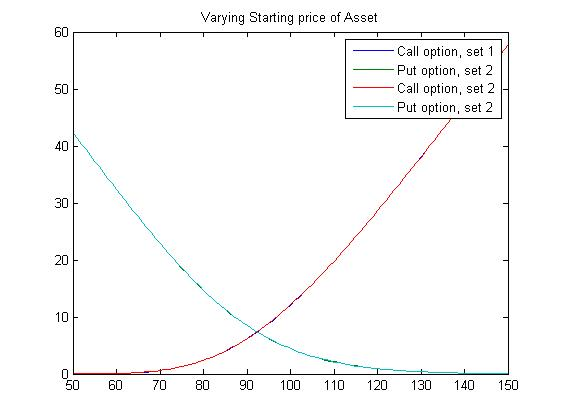
\includegraphics[width=6in]{asset.jpg}
    \end{center}
        \subsubsection*{Dependence on Strike Price}
    \begin{center}
      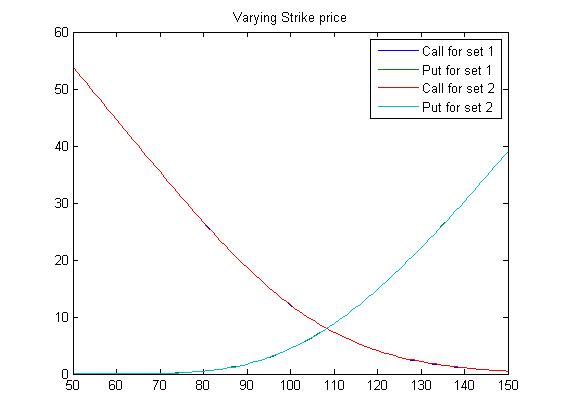
\includegraphics[width=6in]{strike.jpg}
    \end{center}
        \subsubsection*{Dependence on Rate}
    \begin{center}
      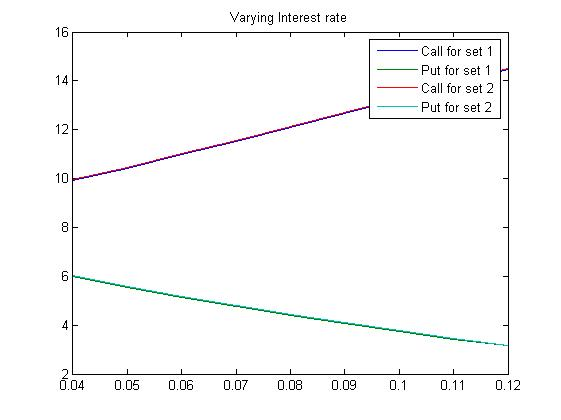
\includegraphics[width=6in]{rate.jpg}
    \end{center}
        \subsubsection*{Dependence on Volatility}
    \begin{center}
      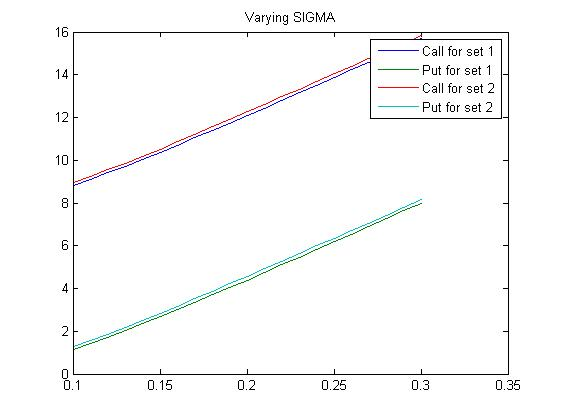
\includegraphics[width=6in]{sigma.jpg}
    \end{center}
    \subsubsection*{Dependence on Number of Steps}
    \begin{center}
      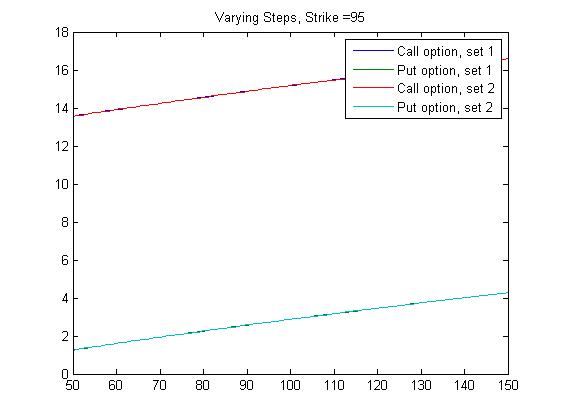
\includegraphics[width=6in]{steps95.jpg}
      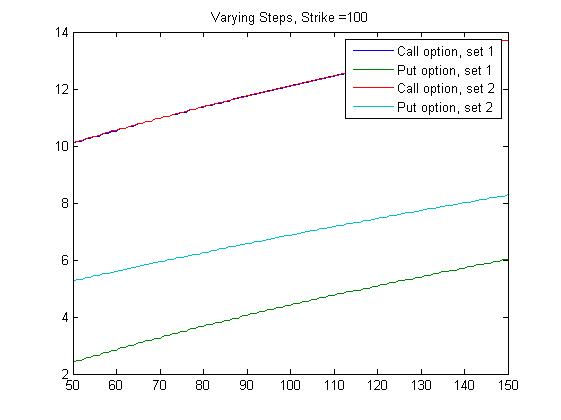
\includegraphics[width=6in]{steps100.jpg}
      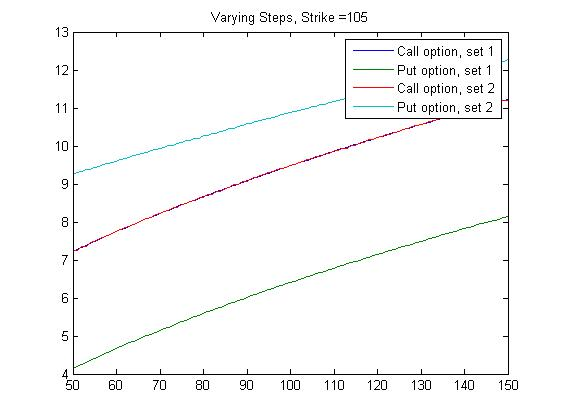
\includegraphics[width=6in]{steps105.jpg}
    \end{center}

\section{Code}
  \subsection{Function for Valuating a European Option}
     \lstinputlisting{european.m}
  \subsection{Code for Analysing European Options}
     \lstinputlisting{lab2.m}

\end{document}

